
%
\section{Combined results}
\label{sec:results}

\begin{figure}[htbp`]
  \centering
\subfigure[]{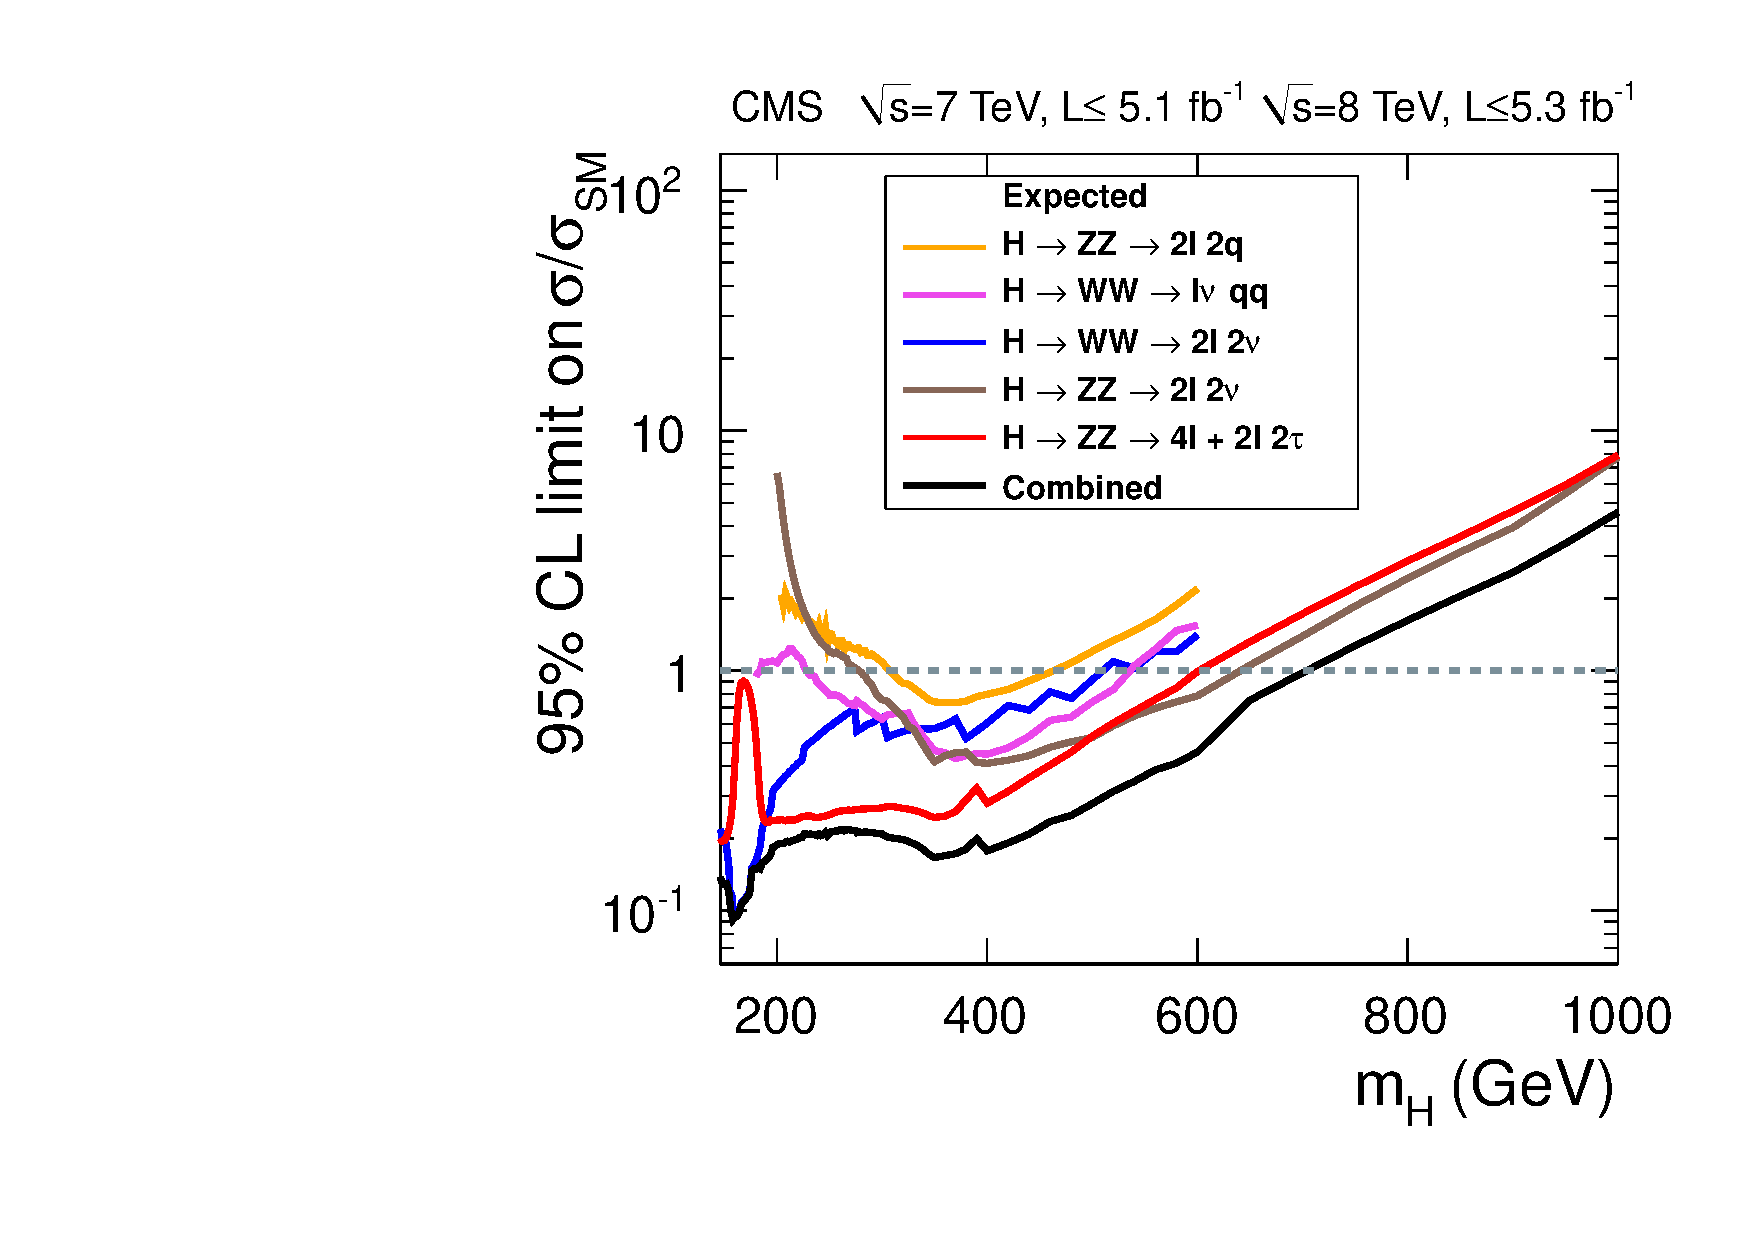
\includegraphics[width=0.45\textwidth]{figures/AllLimitsExpected.pdf}}
\subfigure[]{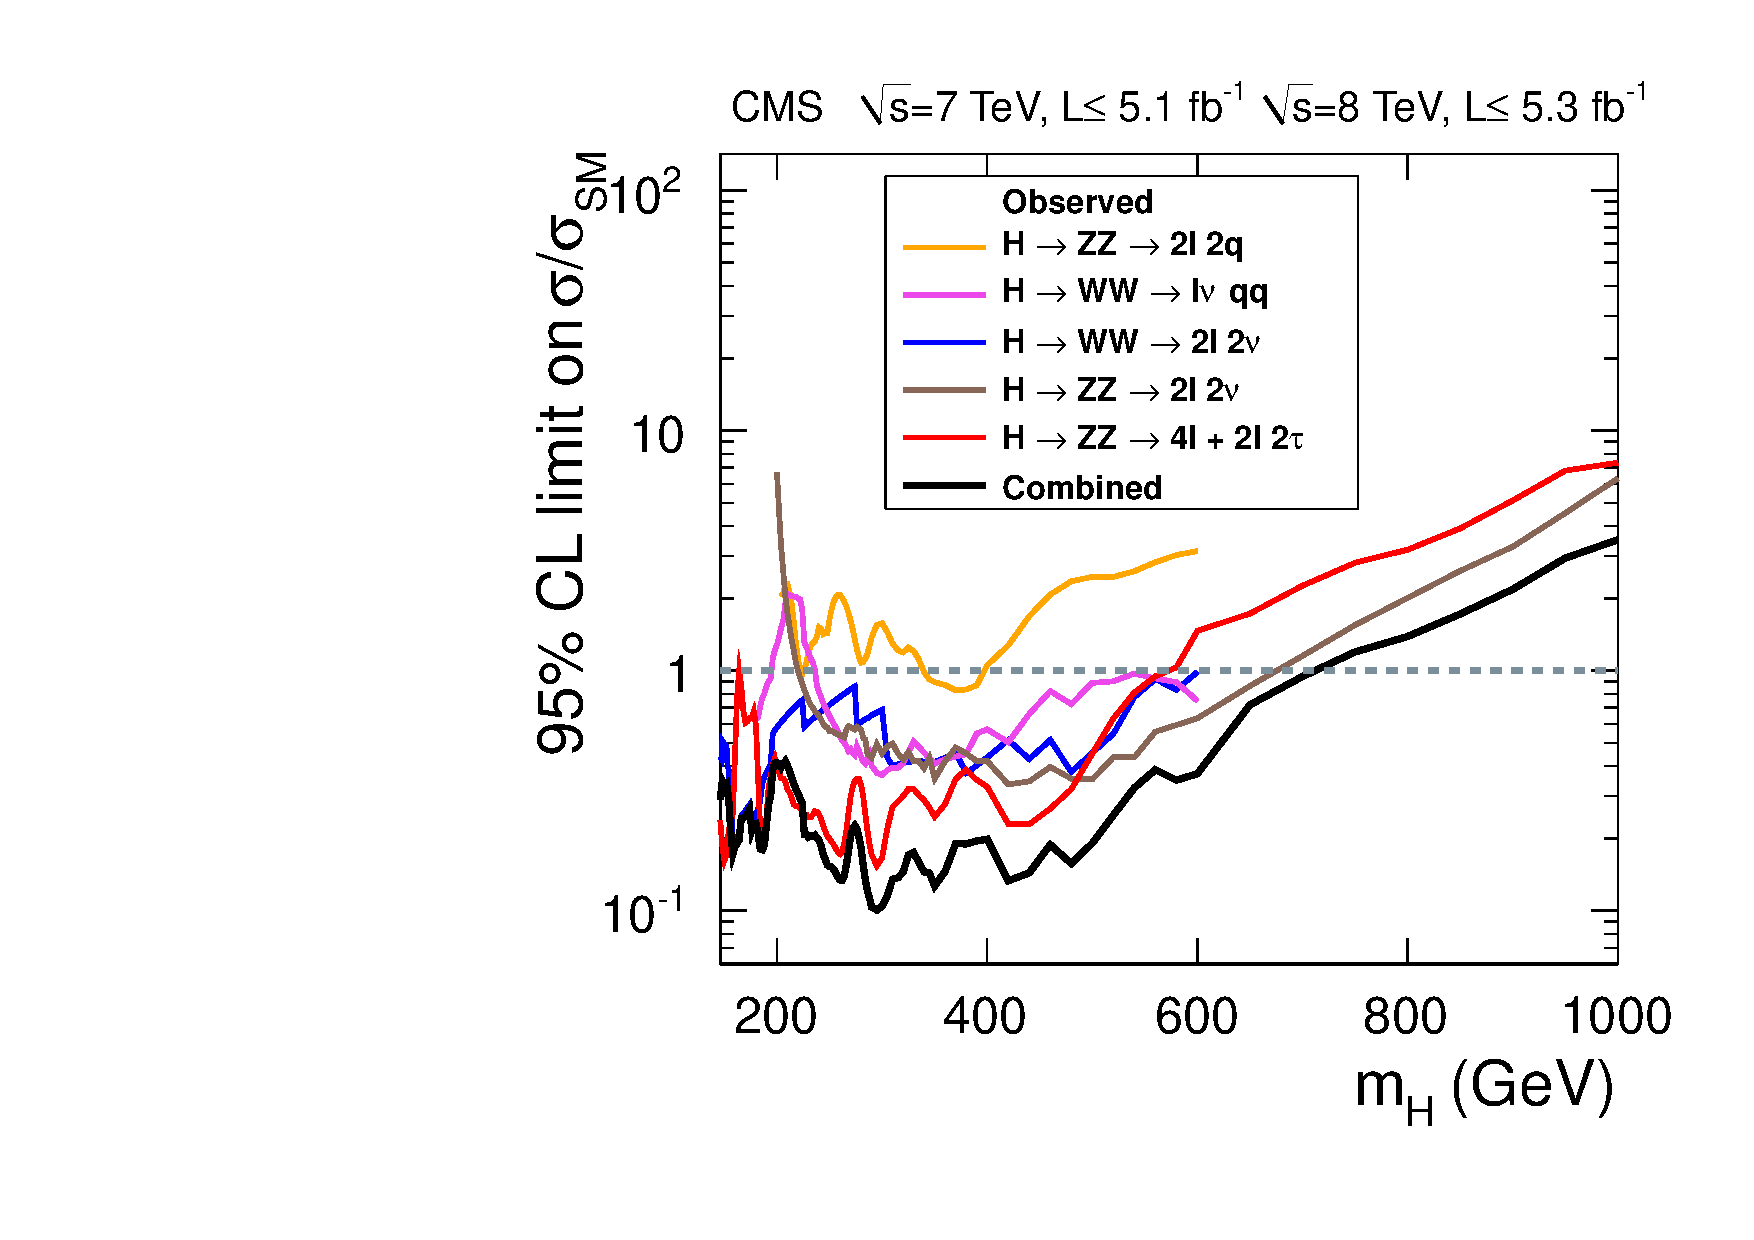
\includegraphics[width=0.45\textwidth]{figures/AllLimitsObserved.pdf}}
  \caption{\label{fig:AllLimits} (a) Expected and  (b) observed 95\% CL limits
  for all individual channels and their combinations.}
\end{figure}

The upper limits on the ratio of the production cross section for the Higgs boson to the SM expectation, for each of the individual channels presented in this paper, are plotted in Figure~\ref{fig:AllLimits} for both expected and
observed limits. This figure also shows a combined limit, calculated using the methods outlined in References~\cite{LHC-HCG-Report, CMScombFeb2012}. The combination procedure assumes the relative branching fractions to be those predicted by the SM, and takes into account the experimental statistical and systematic uncertainties as well as theoretical uncertainties. The combined observed and expected limits are presented together in Figure~\ref{fig:combined}. 
Previously published results exclude the SM Higgs boson in the range $127 < \mH <  600\GeV$~\cite{Chatrchyan:2012tx}. The results of this analysis extend the upper exclusion limit to $\mH < 710\GeV$. For $\mH < 200\GeV$ the most sensitive channel is $\WW \to \ell\nu\ell\nu$. At higher masses the two ZZ decay channels, $\ZZ \to 2\ell 2\ell'$ and $\ZZ \to 2\ell 2\nu$,
define mainly the results of the combination. 
%Since the individual limits are dominated by statistical uncertainties,
%correlations between systematic uncertainties in individual channels do not significant affect the power of the combined
%limit.

\begin{figure}[htbp`]
  \centering
  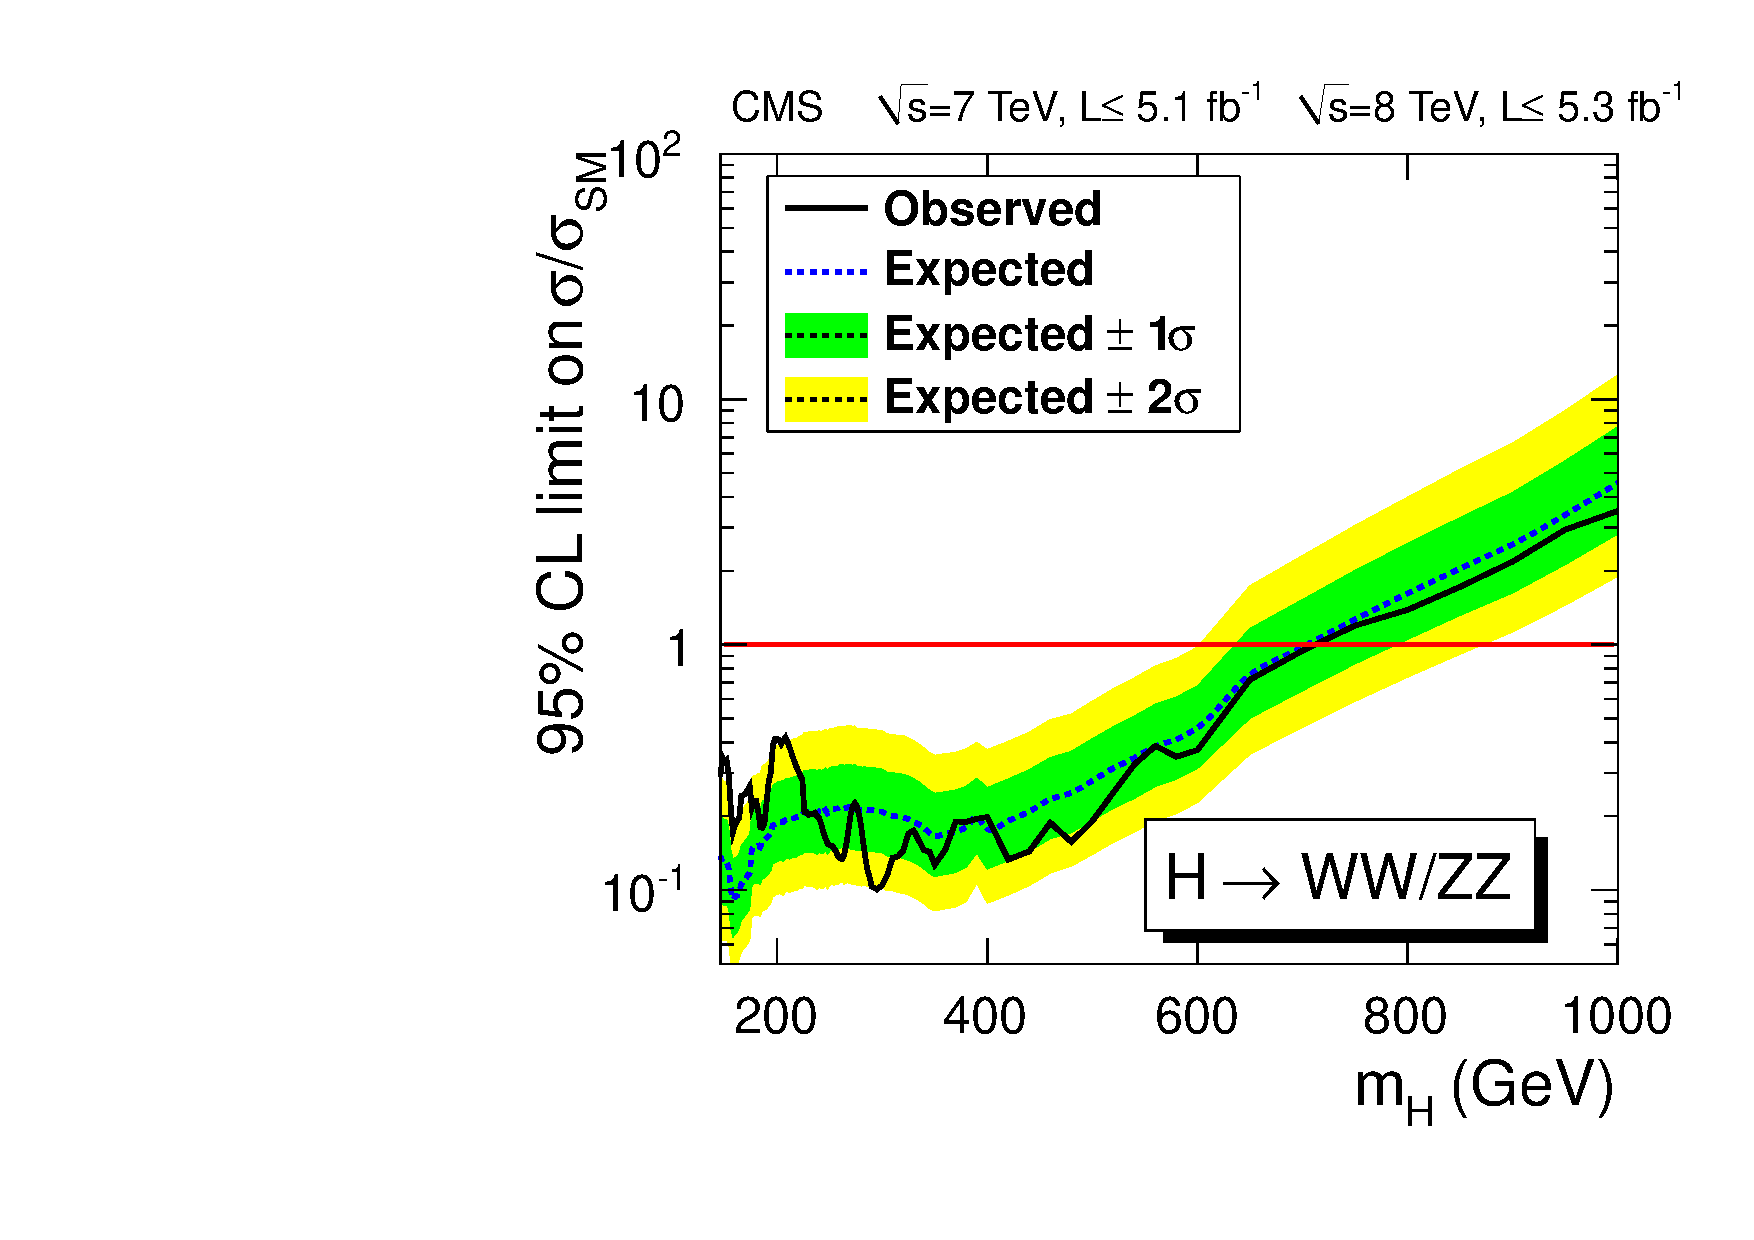
\includegraphics[width=0.6\textwidth]{figures/CombinedLimit.pdf}
  \caption{\label{fig:combined}Observed (solid) and expected
  (dashed) 95\% CL upper limit on the ratio of the production cross
  section to the SM expectation for the Higgs boson with all $\WW$ and $\ZZ$
  channels combined.}
\end{figure}


%%
\section{Summary}
\label{sec:summary}

Results are presented from searches for a standard-model-like Higgs boson in $\PH \to \WW$ and $\PH \to \ZZ$
decay channels, for Higgs boson mass hypotheses in the range $145 < \mH < 1000$ GeV. The analysis uses proton-proton 
collision data recorded by the CMS detector at the LHC, corresponding to integrated luminosities of up to
 5.1 ${\rm fb}^{-1}$ at 
$\sqrt{s} = 7\TeV$ and up to 5.3 ${\rm fb}^{-1}$ at $\sqrt{s} = 8\TeV$. The final states analysed include
two leptons and two neutrinos, $\PH \to \WW \to \ell\nu\ell\nu$ and $\PH \to \ZZ \to 2\ell 2\nu$, a lepton and two jets, 
$\PH \to \WW \to \ell \nu \mathrm{qq}$, two leptons and two jets, $\PH \to \ZZ \to 2\ell \mathrm{q\bar{q}}$,
or four leptons, $\PH \to \ZZ \to 2\ell 2\ell '$, where $\ell = \Pe$ or $\Pgm$ and $\ell ' = \Pe$ or $\Pgm$, or $\Pgt$.
The results  are consistent with the standard model expectations. 
Upper limits at 95\% confidence level exclude a standard-model-like Higgs boson in the range $145 < \mH <  710\GeV$, thus extending the  
mass region excluded by CMS from
$127-600\GeV$ up to $710\GeV$.  
The expected exclusion range $118-543\GeV$ is extended up to $700\GeV$.

%The measured combined
%upper limits at 95\% confidence level on products of the cross-section and branching 
%fractions 
%exclude 
%for the standard-model-like Higgs boson
%extend the mass range excluded by CMS from
%$127<\mH<600\GeV$ to $127<\mH<710\GeV$.
